% ============================================================
\section{Programación}\label{sec:programacion}
% ============================================================

\subsection{Entorno y organización del firmware}
El firmware final (proyecto \texttt{programa/RobotArm}) se desarrolló en C con STM32CubeIDE,
con la configuración de periféricos generada en STM32CubeMX y la biblioteca HAL de
ST~\cite{hal}. El código se organizó en módulos con responsabilidades separadas
(Tabla~\ref{tab:modulos-fw}). El código fuente completo está en el repositorio del
proyecto~\cite{repo} y los fragmentos principales, en el Anexo~\ref{anx:codigo}.

\begin{table}[H]
\centering\small
\caption{Módulos del firmware.}\label{tab:modulos-fw}
\begin{tabularx}{\textwidth}{@{}l X@{}}
\toprule
\textbf{Archivo} & \textbf{Responsabilidad}\\
\midrule
\texttt{main.c} & Inicialización de reloj y periféricos, \emph{super-loop}, \emph{callbacks} HAL de timers y EXTI, refresco del LCD.\\
\texttt{robot\_logic.c} & Intérprete de comandos, modos operativos, máquina de estados, recorte a límites articulares, telemetría y registro de interrupciones.\\
\texttt{motor\_driver.c} & Estructura \texttt{StepperMotor}, generación de pasos en la ISR de TIM2, rampa trapezoidal, \emph{homing}, finales de carrera y parada de emergencia.\\
\texttt{gripper\_driver.c} & PWM del servo: conversión de ángulo a ancho de pulso, apertura y cierre configurables.\\
\texttt{comm\_manager.c} & Transmisión USB CDC con \emph{timeout} y utilidades de análisis de tramas.\\
\texttt{lcd\_i2c.c} & Driver del LCD HD44780 vía PCF8574 con autodetección de dirección.\\
\texttt{robot\_defines.h} & Constantes globales (frecuencia de timer, límites, estados, códigos de IRQ) y estructura de motor.\\
\texttt{stm32f1xx\_it.c} & Vectores de interrupción (TIM2, TIM3, EXTI15\_10, USB).\\
\bottomrule
\end{tabularx}
\end{table}

% ------------------------------------------------------------
\subsection{Configuración del reloj}
Se usa el cristal externo (HSE) de \SI{8}{\mega\hertz} multiplicado por el PLL:
\begin{equation}
  f_{\mathrm{SYSCLK}} = f_{\mathrm{HSE}}\cdot \mathrm{PLLMUL} = \SI{8}{\mega\hertz}\cdot 9 = \SI{72}{\mega\hertz},
  \qquad
  f_{\mathrm{USB}} = \frac{\SI{72}{\mega\hertz}}{1{,}5} = \SI{48}{\mega\hertz}.
\end{equation}
AHB y APB2 trabajan a \SI{72}{\mega\hertz}. APB1 trabaja a \SI{36}{\mega\hertz}, y como su
prescaler es distinto de 1, los timers de APB1 (TIM2, TIM3 y TIM4) reciben el doble,
\SI{72}{\mega\hertz}. La Flash opera con 2 estados de espera. El USB exige exactamente
\SI{48}{\mega\hertz}, lo que condiciona la elección de 72~MHz como frecuencia de sistema.

% ------------------------------------------------------------
\subsection{Configuración de periféricos}
La frecuencia de desborde de un temporizador vale
\begin{equation}
  f_{\mathrm{TIM}} = \frac{f_{\mathrm{CK}}}{(\mathrm{PSC}+1)(\mathrm{ARR}+1)}.
  \label{eq:ftim}
\end{equation}

\begin{table}[H]
\centering\small
\caption{Configuración de periféricos del STM32F103C8T6.}\label{tab:perifericos}
\begin{tabularx}{\textwidth}{@{}l >{\raggedright\arraybackslash}p{6.2cm} >{\raggedright\arraybackslash}X@{}}
\toprule
\textbf{Periférico} & \textbf{Configuración} & \textbf{Uso}\\
\midrule
TIM2 & PSC = 71, ARR = 49 $\Rightarrow$ \SI{20}{\kilo\hertz}; IRQ por desborde & Base de tiempo de la generación de pasos (``metrónomo'' de \SI{50}{\micro\second}).\\
TIM3 & PSC = 7199, ARR = 9999 $\Rightarrow$ \SI{1}{\hertz}; IRQ por desborde & Contador de segundos para supervisión de tiempos.\\
TIM4 & PSC = 71, ARR = 19999 $\Rightarrow$ \SI{50}{\hertz}; CH4 en PWM1 & Señal del servo en PB9, resolución de \SI{1}{\micro\second}.\\
EXTI 12--15 & Entradas con \emph{pull-up}, disparo por flanco; vector EXTI15\_10, prioridad 0 & Finales de carrera X/Y/Z (PB12--PB14) y E-STOP (PB15).\\
GPIO salidas & \emph{Push-pull}, baja velocidad & STEP/DIR (PA0--PA5), ENABLE (PB8), LEDs (PB3--PB5, PC13).\\
I2C1 & Modo estándar, \SI{100}{\kilo\hertz}, direccionamiento de 7 bits & LCD 16$\times$2 (PB6/PB7).\\
USB & Device FS, \emph{middleware} CDC (VCP) & Comunicación con la PC.\\
SYS & Serial Wire Debug, SysTick como base de tiempo de la HAL & Depuración y \texttt{HAL\_GetTick()}.\\
\bottomrule
\end{tabularx}
\end{table}

Aplicando \eqref{eq:ftim}:
\begin{align}
  f_{\mathrm{TIM2}} &= \frac{\SI{72}{\mega\hertz}}{72\cdot 50} = \SI{20}{\kilo\hertz}, &
  f_{\mathrm{TIM3}} &= \frac{\SI{72}{\mega\hertz}}{7200\cdot 10000} = \SI{1}{\hertz}, &
  f_{\mathrm{TIM4}} &= \frac{\SI{72}{\mega\hertz}}{72\cdot 20000} = \SI{50}{\hertz}.
\end{align}

\fig[0.75\textwidth]{cubemx_clock}{Árbol de reloj configurado en STM32CubeMX.}{fig:clock}{captura de la pestaña \emph{Clock Configuration} de \texttt{RobotArm.ioc}}

% ------------------------------------------------------------
\subsection{Generación de pasos}\label{sec:prog-pasos}
Cada motor está representado por una estructura \texttt{StepperMotor} que guarda sus pines,
la posición actual y la de destino (en pasos), el sentido, la velocidad instantánea y la de
objetivo, los parámetros de rampa y un contador de ticks. La ISR de TIM2
(\texttt{Motor\_Timer\_Callback}) se ejecuta cada \SI{50}{\micro\second} y recorre los tres
motores. Para una velocidad $v$ (pasos/s) se calcula el intervalo entero
\begin{equation}
  N = \left\lfloor \frac{f_{\mathrm{TIM2}}}{v} \right\rfloor .
\end{equation}
Cuando el contador del motor alcanza $N$ se fija DIR y se pone STEP en alto. En el tick
siguiente se baja STEP, se actualiza la posición y se recalcula la rampa. El pulso dura
entonces un tick (\SI{50}{\micro\second}) y el período real de paso es de $N+1$ ticks:
\begin{equation}
  f_{\mathrm{paso}} = \frac{f_{\mathrm{TIM2}}}{N+1},
  \qquad
  n_{\mathrm{rpm}} = \frac{60\, f_{\mathrm{paso}}}{\text{pasos por vuelta}} .
\end{equation}
La Tabla~\ref{tab:cuantizacion} muestra la frecuencia efectiva en varios puntos del rango.
El error de cuantización crece con la velocidad (\SI{-4,8}{\percent} a \SI{1000}{pasos/s}).
Para esta aplicación es aceptable, porque la posición se controla contando pasos y no
tiempo, pero justifica la mejora propuesta en la Sección~\ref{sec:conclusiones}.

\begin{table}[H]
\centering\small
\caption{Frecuencia de paso efectiva y velocidad del eje del motor (\ang{1,8}, 200 pasos/vuelta).}\label{tab:cuantizacion}
\begin{tabular}{@{}cccccc@{}}
\toprule
\textbf{Comando} & \textbf{$v$ pedida [pasos/s]} & \textbf{$N$} & \textbf{$f_{\mathrm{paso}}$ [Hz]} & \textbf{Error} & \textbf{RPM motor}\\
\midrule
(mínima de arranque) & 50  & 400 & 49,9  & \SI{-0,2}{\percent} & 15,0\\
\cmd{:-V010}         & 100 & 200 & 99,5  & \SI{-0,5}{\percent} & 29,9\\
(por defecto)        & 300 & 66  & 298,5 & \SI{-0,5}{\percent} & 89,6\\
\cmd{:-V050}         & 500 & 40  & 487,8 & \SI{-2,4}{\percent} & 146,3\\
\cmd{:-V100}         & 1000& 20  & 952,4 & \SI{-4,8}{\percent} & 285,7\\
\bottomrule
\end{tabular}
\end{table}

\noindent La velocidad global del comando \cmd{:-Vnnn} (10 a 100~\%) se traduce como
$v = 10\cdot\% $ pasos/s. En la práctica la velocidad queda acotada al rango
\SIrange{50}{1000}{pasos/s}, porque una consigna menor que la de arranque se eleva a
$v_{\min}=\SI{50}{pasos/s}$.

La Figura~\ref{fig:flujo-isr} muestra el diagrama de flujo de la ISR. Antes de generar un
pulso verifica, en orden de prioridad, el E-STOP, el final de carrera en el sentido de
avance y el límite articular opuesto.

\begin{figure}[!htbp]
\centering
\begin{tikzpicture}[node distance=0.5cm]
  \node[terminal] (in) {ISR TIM2 (cada \SI{50}{\micro\second})};
  \node[decision, below=of in] (es) {¿E-STOP?};
  \node[terminal, right=1.2cm of es] (ret) {Retorno};
  \node[proceso, below=0.6cm of es] (for) {Para cada motor $i=0..2$};
  \node[decision, below=of for] (fc) {¿Sensor presionado\\ y avanza hacia él?};
  \node[proceso, right=1.0cm of fc, text width=2.6cm] (stop1) {Frenar eje $i$\\ (\texttt{stepInterval}=0)};
  \node[decision, below=0.6cm of fc] (lim) {¿Calibrado y\\ pos $\ge$ MAX$_i$?};
  \node[proceso, right=1.0cm of lim, text width=2.6cm] (stop2) {Frenar eje $i$,\\ meta = pos actual};
  \node[decision, below=0.6cm of lim] (act) {¿Eje activo?};
  \node[proceso, below=of act] (cnt) {\texttt{stepCounter++}};
  \node[decision, below=of cnt] (hi) {¿cnt $\ge N$?};
  \node[proceso, right=1.0cm of hi, text width=2.6cm] (sh) {DIR, STEP = 1};
  \node[decision, below=0.6cm of hi] (lo) {¿cnt $\ge N{+}1$?};
  \node[proceso, right=1.0cm of lo, text width=2.9cm] (sl) {STEP = 0, cnt = 0\\ pos $\pm$= 1\\ \texttt{CalculateSpeed}};
  \node[proceso, below=0.6cm of lo] (next) {Siguiente motor};
  \draw[flecha] (in) -- (es);
  \draw[flecha] (es) -- node[above,font=\scriptsize]{sí} (ret);
  \draw[flecha] (es) -- node[right,font=\scriptsize]{no} (for);
  \draw[flecha] (for) -- (fc);
  \draw[flecha] (fc) -- node[above,font=\scriptsize]{sí} (stop1);
  \draw[flecha] (fc) -- node[right,font=\scriptsize]{no} (lim);
  \draw[flecha] (lim) -- node[above,font=\scriptsize]{sí} (stop2);
  \draw[flecha] (lim) -- node[right,font=\scriptsize]{no} (act);
  \draw[flecha] (act) -- node[right,font=\scriptsize]{sí} (cnt);
  \draw[flecha] (cnt) -- (hi);
  \draw[flecha] (hi) -- node[above,font=\scriptsize]{sí} (sh);
  \draw[flecha] (hi) -- node[right,font=\scriptsize]{no} (lo);
  \draw[flecha] (sh.south) -- ++(0,-0.3) -| ($(lo.north)+(0.9,0)$);
  \draw[flecha] (lo) -- node[above,font=\scriptsize]{sí} (sl);
  \draw[flecha] (lo) -- node[right,font=\scriptsize]{no} (next);
  \draw[flecha] (sl.south) |- (next.east);
  \draw[flecha] (act.west) -- node[above,font=\scriptsize]{no} ++(-1.4,0) |- (next.west);
  \draw[flecha] (stop1.east) -- ++(0.4,0) |- ($(next.east)+(0,-0.15)$);
  \draw[flecha] (stop2.east) -- ++(0.3,0) |- ($(next.east)+(0,-0.15)$);
  \draw[flecha] (next.west) -- ++(-2.0,0) |- (for.west);
\end{tikzpicture}
\caption{Diagrama de flujo de la rutina de interrupción de TIM2 (generación de pasos).}\label{fig:flujo-isr}
\end{figure}

% ------------------------------------------------------------
\subsection{Perfil de velocidad trapezoidal}
Para evitar la pérdida de pasos en el arranque y en la frenada, en cada paso se recalcula la
velocidad (\texttt{CalculateSpeed}) con incrementos constantes $a=\SI{5}{pasos/s}$ por paso,
partiendo de $v_{\min}=\SI{50}{pasos/s}$:
\begin{equation}
  v_{k+1} =
  \begin{cases}
    \max(v_k - a,\ v_{\min}) & \text{si } d_k \le n_{\mathrm{fr}} = \dfrac{v_k - v_{\min}}{a} \quad\text{(frenado)}\\[6pt]
    \min(v_k + a,\ v_t) & \text{si } v_k < v_t \quad\text{(aceleración)}\\[4pt]
    v_k & \text{en otro caso (crucero)}
  \end{cases}
\end{equation}
donde $d_k$ es la cantidad de pasos restantes y $v_t$ la velocidad objetivo. El número de
pasos y el tiempo necesarios para acelerar hasta $v_t$ resultan
\begin{equation}
  n_{\mathrm{acc}} = \frac{v_t - v_{\min}}{a},
  \qquad
  t_{\mathrm{acc}} = \sum_{k=0}^{n_{\mathrm{acc}}-1}\frac{1}{v_{\min}+k\,a}
  \;\approx\; \frac{1}{a}\ln\frac{v_t}{v_{\min}} .
\end{equation}
Para $v_t=\SI{1000}{pasos/s}$: $n_{\mathrm{acc}}=190$ pasos y $t_{\mathrm{acc}}\approx\SI{0,60}{\second}$.
Si el recorrido $d$ es menor que $2n_{\mathrm{acc}}$, el perfil queda triangular y la
velocidad pico es $v_{\mathrm{pico}}\approx v_{\min}+a\,d/2$. Con los recorridos máximos de los
ejes Y (130 pasos) y Z (60 pasos), los picos son de 375 y \SI{200}{pasos/s}, respectivamente:
en esos ejes la rampa, y no el comando de velocidad, limita la velocidad alcanzable
(Figura~\ref{fig:rampa}).

\begin{figure}[!htbp]
\centering
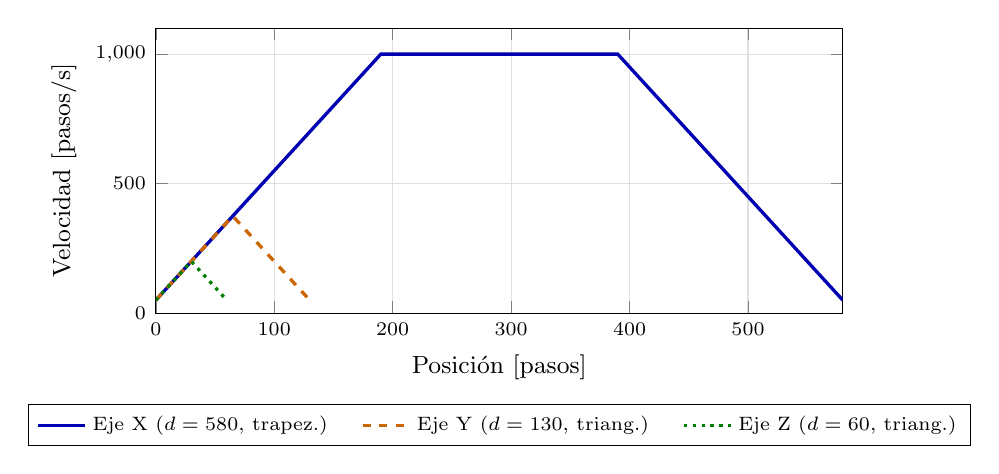
\begin{tikzpicture}
\begin{axis}[width=0.85\textwidth, height=5.2cm, xlabel={Posición [pasos]}, ylabel={Velocidad [pasos/s]},
  xmin=0, xmax=580, ymin=0, ymax=1100, grid=major, grid style={gray!25},
  legend style={font=\scriptsize, at={(0.5,-0.32)}, anchor=north,
                /tikz/every even column/.append style={column sep=0.35cm}},
  legend columns=3, tick label style={font=\scriptsize}, label style={font=\small}]
  \addplot[very thick, blue!70!black] coordinates {(0,50) (190,1000) (390,1000) (580,50)};
  \addlegendentry{Eje X ($d=580$, trapez.)}
  \addplot[very thick, orange!80!black, dashed] coordinates {(0,50) (65,375) (130,50)};
  \addlegendentry{Eje Y ($d=130$, triang.)}
  \addplot[very thick, green!50!black, dotted] coordinates {(0,50) (30,200) (60,50)};
  \addlegendentry{Eje Z ($d=60$, triang.)}
\end{axis}
\end{tikzpicture}
\caption{Perfiles de velocidad teóricos para un recorrido completo de cada eje a velocidad global de 100~\%.}\label{fig:rampa}
\end{figure}

% ------------------------------------------------------------
\subsection{Rutina de \emph{homing}}\label{sec:prog-homing}
\texttt{HomingMotors} referencia los ejes de forma secuencial: primero Y (hombro), para
levantar el brazo; luego Z (codo), para recogerlo, y por último X (base), para no barrer el
área de trabajo con el brazo extendido. Se usan velocidades bajas y constantes: 60 pasos/s en
X e Y y 30 pasos/s en Z. Si un sensor ya está presionado al comenzar, el eje primero retrocede
hasta liberarlo (\emph{smart homing}). Terminada la búsqueda, los tres ejes retroceden a la
vez unos pasos (\emph{back-off}) para liberar los sensores y se fija la posición cero
(Figura~\ref{fig:flujo-homing}). Las esperas usan \texttt{HAL\_GetTick()} (SysTick) como
referencia de tiempo y llaman a un latido que mantiene la telemetría activa. Cada salida con
error devuelve un código que el firmware traduce a un mensaje (Tabla~\ref{tab:err-homing}).

\paragraph{Tiempos medidos y ajuste del \emph{timeout}.}
Con el robot montado se midió la duración de cada tramo del \emph{homing}: \SI{3,53}{\second} el
eje Y, \SI{1,19}{\second} el eje Z y \SI{10,87}{\second} el eje X, lo que da un \emph{homing}
completo de \SI{15,59}{\second}. El eje X es el más lento porque recorre todo su rango
(580 pasos a \SI{60}{pasos/s}). Con el \emph{timeout} de búsqueda original de \SI{10}{\second}
por eje se detectó un defecto: en el caso más desfavorable el eje X \emph{alcanzaba} el final de
carrera pero el temporizador expiraba un instante antes, de modo que el \emph{homing} terminaba
físicamente bien pero el firmware reportaba un error de \emph{timeout}. Se corrigió haciendo el
\emph{timeout} de búsqueda dependiente del eje: \SI{10}{\second} para Y y Z, y \SI{16}{\second}
para X, con holgura sobre el peor caso medido.

\begin{figure}[!htbp]
\centering
\begin{tikzpicture}[node distance=0.45cm]
  \node[terminal] (s) {\cmd{:-H}};
  \node[proceso, below=of s] (en) {Habilitar drivers, abrir pinza};
  \node[proceso, below=of en] (ax) {Eje siguiente: Y $\rightarrow$ Z $\rightarrow$ X};
  \node[decision, below=of ax] (pr) {¿Sensor ya\\ presionado?};
  \node[proceso, right=1.0cm of pr, text width=3.0cm] (bo) {Alejarse hasta liberar\\ (timeout \SI{5}{\second})};
  \node[proceso, below=0.55cm of pr, text width=3.8cm] (bus) {Avanzar hacia el sensor a velocidad constante};
  \node[decision, below=of bus] (ok) {¿Sensor, E-STOP\\ o \emph{timeout}?};
  \node[proceso, right=1.0cm of ok, text width=3.0cm, fill=red!8] (err) {Error: timeout / sensor trabado / abortado};
  \node[decision, below=0.55cm of ok] (last) {¿Quedan ejes?};
  \node[proceso, below=0.55cm of last, text width=3.8cm] (back) {\emph{Back-off} simultáneo (5 pasos; Z: 2)};
  \node[proceso, below=of back, text width=3.8cm] (zero) {Posición = 0, calibrado = 1\\ LEDs HOME y FINISH};
  \node[terminal, below=of zero] (fin) {Homing OK};
  \draw[flecha] (s) -- (en); \draw[flecha] (en) -- (ax); \draw[flecha] (ax) -- (pr);
  \draw[flecha] (pr) -- node[above,font=\scriptsize]{sí} (bo);
  \draw[flecha] (bo) |- (bus.east);
  \draw[flecha] (pr) -- node[right,font=\scriptsize]{no} (bus);
  \draw[flecha] (bus) -- (ok);
  \draw[flecha] (ok) -- node[above,font=\scriptsize]{E-STOP / t} (err);
  \draw[flecha] (ok) -- node[right,font=\scriptsize]{sensor} (last);
  \draw[flecha] (last.west) -- node[above,font=\scriptsize]{sí} ++(-1.3,0) |- (ax.west);
  \draw[flecha] (last) -- node[right,font=\scriptsize]{no} (back);
  \draw[flecha] (back) -- (zero); \draw[flecha] (zero) -- (fin);
\end{tikzpicture}
\caption{Diagrama de flujo de la rutina de \emph{homing}.}\label{fig:flujo-homing}
\end{figure}

\begin{table}[H]
\centering\small
\caption{Códigos de error del \emph{homing}.}\label{tab:err-homing}
\begin{tabular}{@{}cl@{}}
\toprule
\textbf{Código} & \textbf{Significado}\\
\midrule
$-1$, $-2$, $-3$ & Eje X, Y o Z no encontró su final de carrera (\emph{timeout} de búsqueda: \SI{16}{\second} en X, \SI{10}{\second} en Y/Z)\\
$-11$, $-12$, $-13$ & Eje X, Y o Z: el final de carrera no se libera (sensor o mecánica)\\
$-9$ & Homing abortado por parada de emergencia\\
\bottomrule
\end{tabular}
\end{table}

% ------------------------------------------------------------
\subsection{Finales de carrera y parada de emergencia (EXTI)}
Las cuatro entradas comparten el vector \texttt{EXTI15\_10\_IRQn}, configurado con la
prioridad más alta. El \emph{callback} \texttt{Motor\_Sensor\_Triggered} distingue el pin de
origen:
\begin{itemize}
  \item \textbf{E-STOP (PB15):} llama a \texttt{Motor\_EmergencyStop()}, que anula velocidad e
        intervalo de los tres ejes y fija \texttt{robotState = STATE\_ESTOP}. El comando
        \cmd{:-S} ejecuta la misma función, así que ambas vías tienen idéntica respuesta.
  \item \textbf{Final de carrera:} detiene sólo el eje afectado y da su meta por alcanzada en
        la posición actual. Así se evita que un destino más allá del sensor deje el movimiento
        ``pendiente'' y lo vuelva a lanzar con cada comando siguiente.
\end{itemize}
Dentro de la ISR no se transmite por USB, porque la transmisión puede demorar hasta
\SI{10}{\milli\second}. Se registra el origen en \texttt{lastIrqSource} y el lazo principal
emite el mensaje (\texttt{IRQ|E-STOP: boton fisico (PB15)}, \texttt{IRQ|Fin de carrera: eje X
(PB12)}, etc.).

% ------------------------------------------------------------
\subsection{PWM del servo de la pinza}\label{sec:prog-pwm}
Con TIM4 contando a $f_{\mathrm{CK}}/(\mathrm{PSC}+1)=\SI{1}{\mega\hertz}$, cada unidad del
registro de comparación equivale a \SI{1}{\micro\second}. El ángulo $\theta\in[\ang{0},\ang{180}]$
se convierte en el valor del registro CCR4 con
\begin{equation}
  \mathrm{CCR4}(\theta) = P_{\min} + \frac{\theta\,(P_{\max}-P_{\min})}{180}
  = 550 + \frac{1900\,\theta}{180}\ [\si{\micro\second}],
\end{equation}
que da una resolución de $\ang{180}/1900 \approx \ang{0,095}$ por cuenta y un ciclo de trabajo
de \SIrange{2,75}{12,25}{\percent}. El canal arranca con $P_{\min}$ para que el servo reciba
desde el inicio un pulso válido. Los ángulos de apertura (\cmd{:-A}) y cierre (\cmd{:-P}) se
guardan en variables del driver y por defecto valen \ang{90} y \ang{0}.

% ------------------------------------------------------------
\subsection{Comunicación USB e intérprete de comandos}
El periférico USB funciona como dispositivo CDC (puerto COM virtual). El sistema operativo lo
reconoce sin drivers adicionales y la velocidad de transferencia es la del USB Full Speed,
independiente de los baudios que configure la PC. En la ISR de recepción
(\texttt{CDC\_Receive\_FS}) la trama se copia a \texttt{buffer\_rx} y se levanta
\texttt{flagUsb}. Sólo el comando \cmd{:-S} se atiende ahí mismo, para que la parada por
software actúe aun durante el \emph{homing}, que es bloqueante.

\texttt{Robot\_ProcesarComando} primero verifica el enclavamiento: en E-STOP sólo acepta
\cmd{:-R}. Después despacha según el segundo carácter (\cmd{-}, \cmd{\#}, \cmd{+}, \cmd{*}).
Los valores numéricos se extraen con \texttt{BuscarValor(letra, trama)}, que ubica la letra
y convierte los dígitos siguientes con \texttt{atoi}. Por eso el orden de los campos en la
trama es libre y cada eje es opcional. Si el robot está calibrado, cada destino se recorta a
$[0,\mathrm{MAX}_i]$ y se avisa por consola.

\paragraph{Telemetría.}
\texttt{Robot\_UpdateTelemetry} se evalúa cada \SI{50}{\milli\second} y transmite
\begin{center}
\texttt{STATUS|X:<x>|Y:<y>|Z:<z>|S:<sx><sy><sz>|C:<0/1>|M:<0/1>|E:<0/1>}
\end{center}
sólo si cambió la posición, algún sensor, la calibración, el estado de movimiento o el de
E-STOP, y además cada \SI{2}{\second} como señal de vida (\emph{heartbeat}). La misma función
maneja los LEDs WAIT (en movimiento), FINISH (encendido al terminar un movimiento) y HOME
(calibrado, o parpadeo si el \emph{homing} falló).

% ------------------------------------------------------------
\subsection{Interfaz gráfica de PC}
La aplicación \tails{} (Python 3.11, PyQt5, pySerial)~\cite{pyqt,pyserial} sigue el patrón MVC
(Figura~\ref{fig:mvc}). Sus aspectos principales son:
\begin{itemize}
  \item \textbf{Recepción en un hilo dedicado} (\texttt{SerialWorker}, \texttt{QThread}). El hilo
        escucha el puerto sin congelar la interfaz y emite una señal por cada trama. El
        \emph{parser} de telemetría está protegido contra tramas corruptas.
  \item \textbf{Aprendizaje:} el \emph{jogging} se hace con botones o con el teclado
        ($\leftarrow$/$\rightarrow$ para X, $\uparrow$/$\downarrow$ para Y, \texttt{W}/\texttt{S} para Z,
        \texttt{Esc} para parada) y está acotado a los rangos de los ejes. Los puntos capturados
        se cargan en una tabla editable (coordenadas, pinza, velocidad, espera y nombre) que
        permite reordenar filas y valida cada celda.
  \item \textbf{Rutinas JSON:} cada paso es un objeto con destino (\texttt{x}, \texttt{y},
        \texttt{z}), pinza (\texttt{g}), velocidad (\texttt{v}, 10--100~\%), espera (\texttt{t},
        0--\SI{60}{\second}) y nombre (\texttt{n}) (ejemplo en el Anexo~\ref{anx:protocolo}).
        Las claves opcionales toman valores por defecto, de modo que se mantiene la
        compatibilidad con rutinas antiguas.
  \item \textbf{Ejecución:} un \texttt{QTimer} de disparo único envía un paso cada
        \SI{1,5}{\second} más la espera \texttt{t} del punto y actualiza la barra de progreso y
        el registro. Si la telemetría informa \texttt{E:1}, la secuencia se detiene sola.
  \item \textbf{Diagnóstico:} el panel de test usa los comandos \cmd{:*}, la terminal es
        acoplable para enviar comandos manuales, y se puede consultar la ayuda del firmware
        (\cmd{:-?}).
\end{itemize}

\fig[0.9\textwidth]{gui_calibracion}{Interfaz gráfica: pestaña de Calibración.}{fig:gui-cal}{\texttt{interfaz/images/Calibración/calibration.png}}
\fig[0.9\textwidth]{gui_aprendizaje}{Interfaz gráfica: pestaña de Aprendizaje con la tabla de puntos.}{fig:gui-learn}{\texttt{interfaz/images/Aprendizaje/learn.png}}
\fig[0.9\textwidth]{gui_ejecucion}{Interfaz gráfica: pestaña de Ejecución de rutinas.}{fig:gui-run}{\texttt{interfaz/images/Ejecución/execution.png}}
